\subsection{Database Design}
\subsubsection{Database Overview}
\begin{center}
  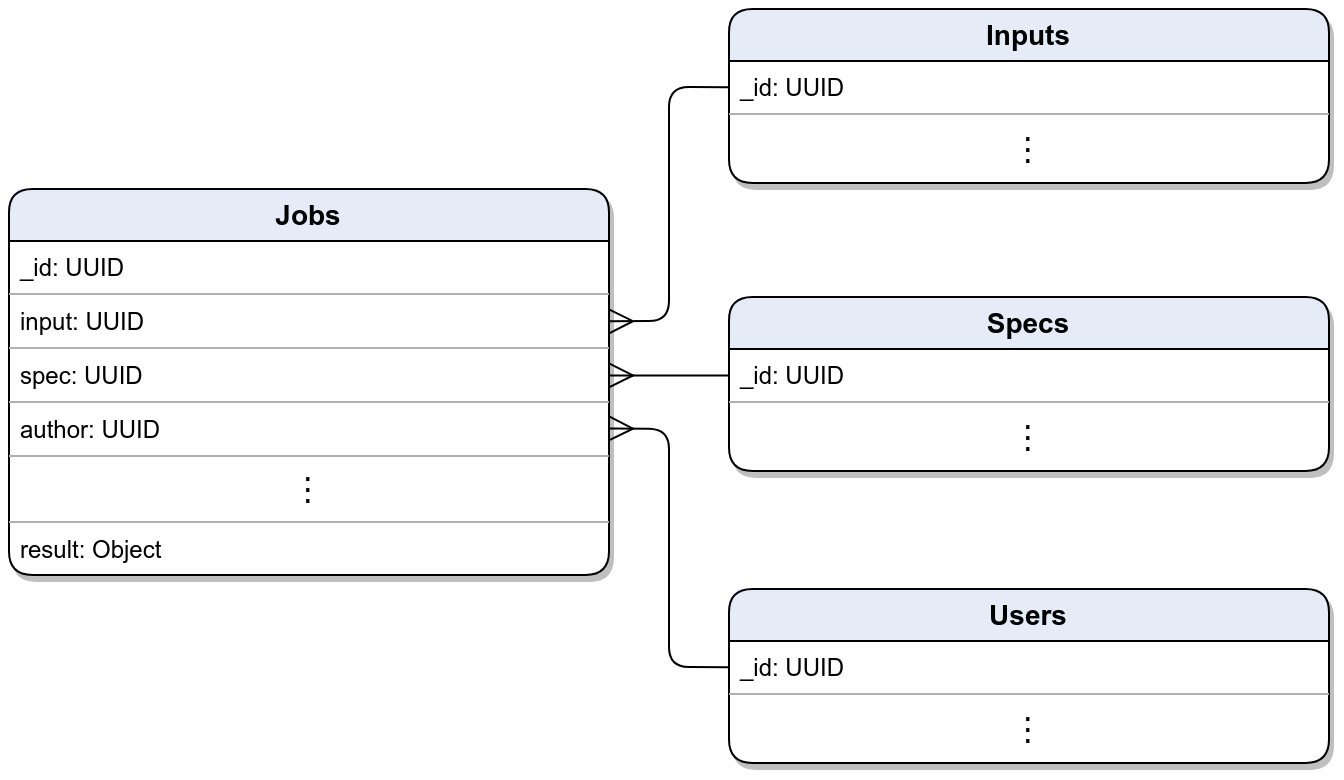
\includegraphics[width=\textwidth]{DatabaseOverview} \\[12pt]
\end{center}
The diagram above represents the database implementation that will be used in the server application at a high level---more detailed representations will follow in the sections below. Note that while this is an entity-relationship diagram, a type of diagram normally used to represent relational databases, a non-relational database (MongoDB) will be used for this application. The ERD, while an imperfect representation for a non-relational database, simply provides a convenient way of demonstrating the format in which information will be stored in collections and the ways in which these collections will relate to one another.\par
There are five collections that will be used to store all information in the database: Jobs, Inputs, Specs, Users, and Groups. The Jobs collection is at the core of the design, as jobs are where the action happens. This collection contains the UUIDs of each relevant document from other collections, metadata about each job, and, upon completion of the job, the resulting output from the analysis performed. The Inputs collection contains information about the WAV audio files to be processed by each job, including the location in which each of the files is stored on the server. The Specs collection holds information about how to process each job, namely, the list of parameters needed for each metric to be run. The Users and Groups collections contain information necessary in keeping track of users and groups.\par

\subsubsection{Jobs, Inputs, \& Specifications}
\begin{center}
  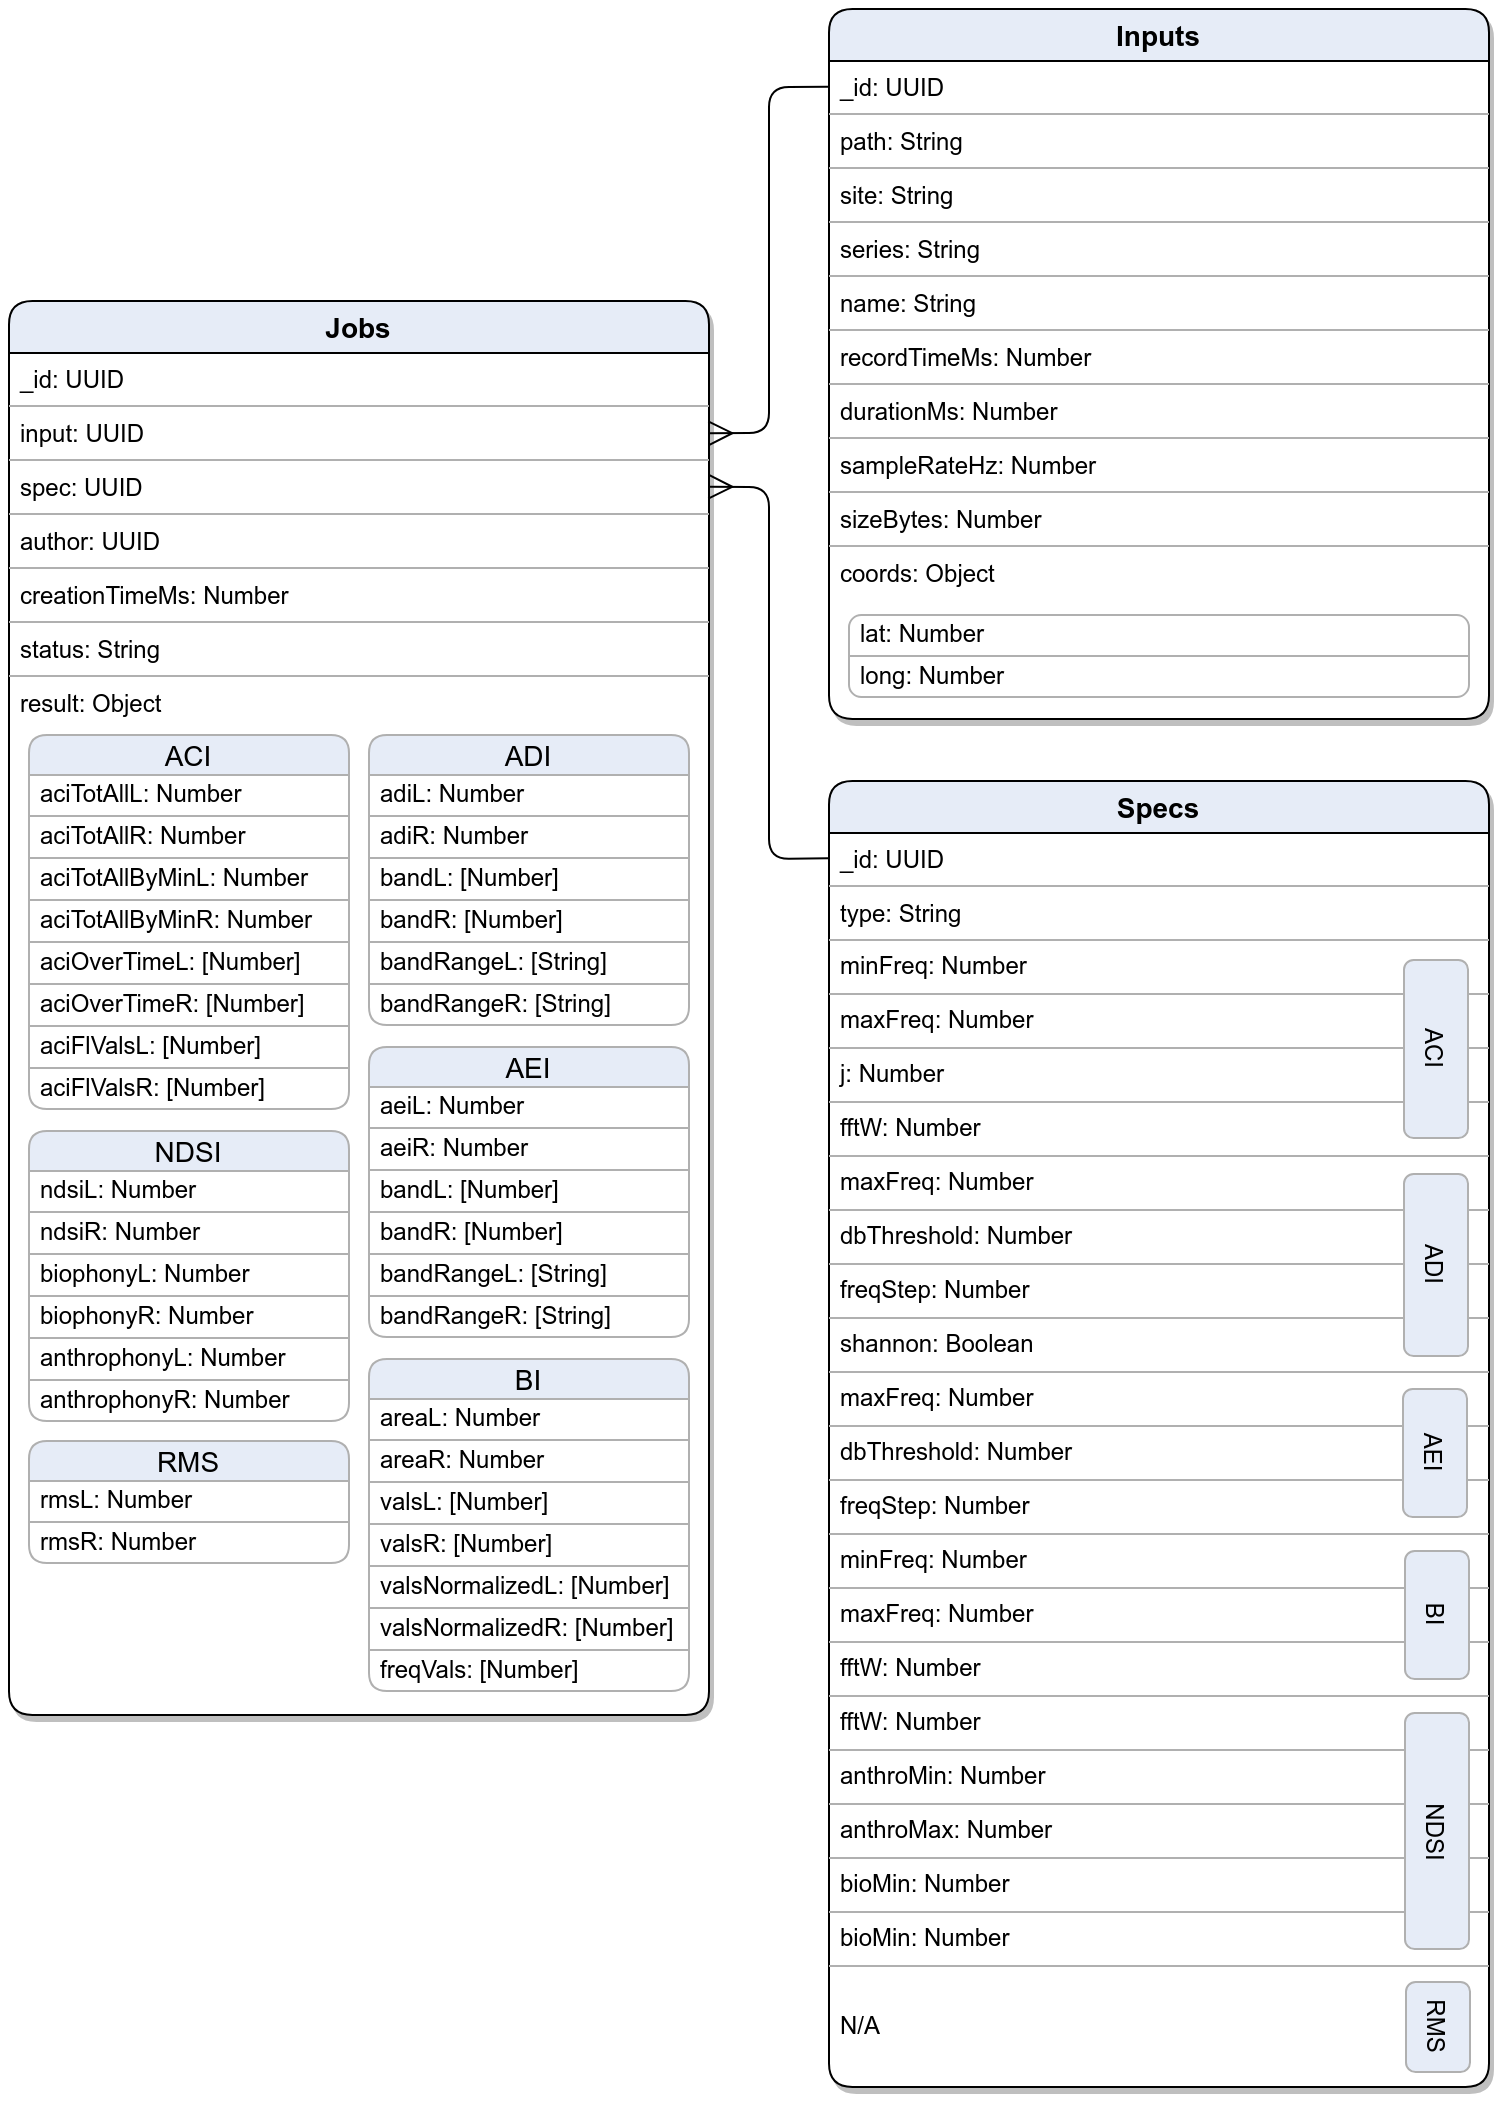
\includegraphics[width=\textwidth]{DatabaseJobs} \\[12pt]
\end{center}
% It should be clear from the diagram that the database design is focused around the Jobs collection, and this makes sense given that jobs are where the action takes place. The Jobs collection connects to
As mentioned, jobs have a start and end time and date for use in creating graphs comparing results over time. In addition to these fields, jobs also have a reference to a fileMetadata object. The way that we have set up our database is that of an M to N relationship, where many jobs can be mapped to many different input sets.\par
The metric data collection represents the parameters used in each job. These parameters are index specific and job specific. We are deciding to keep track of these because it may be useful if the user wants to run the same job on a different data set, that way we are not storing redundant data.\par
These jobs produce outputs, as outlined in the job results collections. Each index has specific outputs based on what they are measuring. These output collections include references to the jobs and data sets that produced them.\par

\subsubsection{Users \& Groups}
\begin{center}
  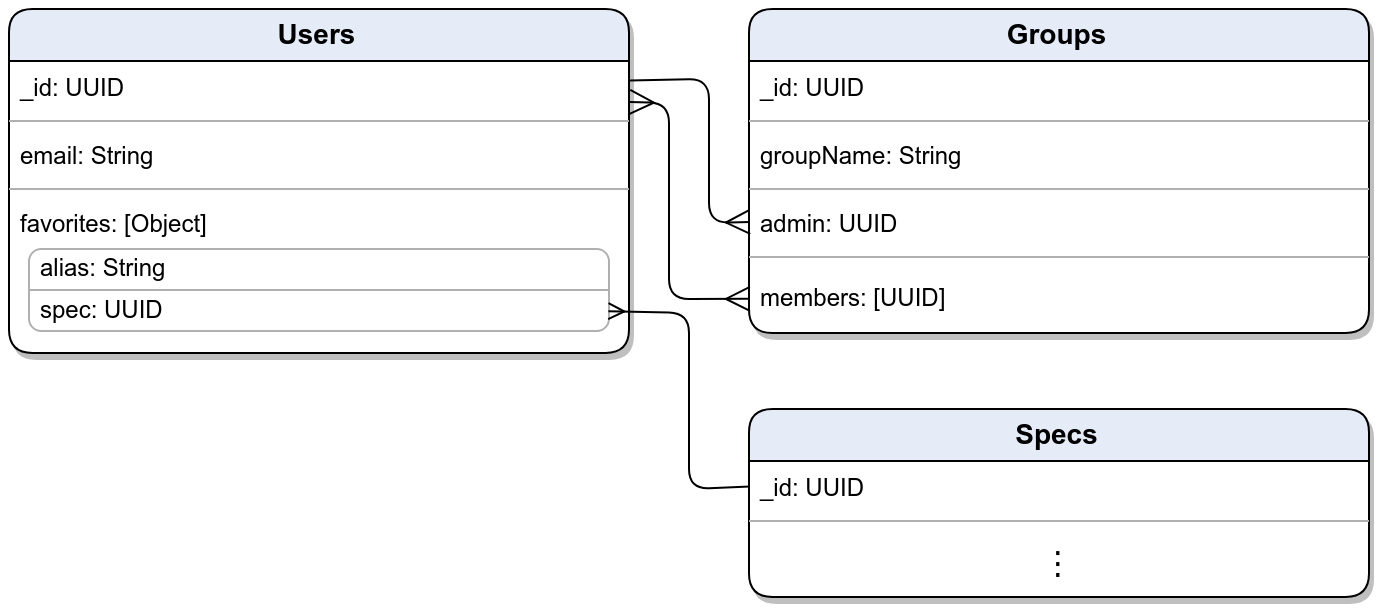
\includegraphics[width=\textwidth]{DatabaseUsers} \\[12pt]
\end{center}
A user signs up for our service using their email address and a password which is hashed and stored in our database. The users then have a few options.\par
First, users can be a part of groups, or create a group. If a user creates a group, they are added as the admin of the group. An admin of a group can then add more users to also be admins. Groups have a list of members as well, referencing the users collection.\par
Second, users can create jobs. These jobs have unique IDs as well as date of completion and the starting date and times. These jobs go into a bit more depth in the next section.
